\documentclass[border=4pt]{standalone}
\usepackage[T1]{fontenc}
\usepackage{tikz}
\usetikzlibrary{arrows.meta,positioning,fit,backgrounds,shapes.geometric,calc}
\definecolor{orch}{HTML}{234767}
\definecolor{ctx}{HTML}{EAF1F8}
\definecolor{retr}{HTML}{E2F0ED}
\definecolor{ext}{HTML}{F7EBDD}
\definecolor{infra}{HTML}{F1F3F5}
\tikzset{
 every node/.style={font=\sffamily\fontsize{8.5}{10}\selectfont,align=center,execute at begin node={\hyphenpenalty=10000\exhyphenpenalty=10000}},
 block/.style={draw=orch!80,fill=white,rounded corners=1.5pt,minimum height=7mm,inner sep=3pt,line width=.55pt},
 context/.style={block,fill=ctx},
 engine/.style={block,fill=orch,text=white},
 retrieval/.style={block,fill=retr},
 external/.style={block,fill=ext},
 storage/.style={block,fill=infra},
 optional/.style={dashed},
 flow/.style={-{Stealth[length=2mm]},draw=orch!90,line width=.65pt},
 control/.style={flow,dashed},
 error/.style={flow,densely dotted},
 group/.style={draw=orch!50,rounded corners=3pt,inner sep=5pt,line width=.5pt},
 heading/.style={font=\sffamily\bfseries\fontsize{8.5}{10}\selectfont,text=orch},
 edgelabel/.style={font=\sffamily\fontsize{7.5}{9}\selectfont,fill=white,inner sep=1pt,text=orch}
}

\begin{document}
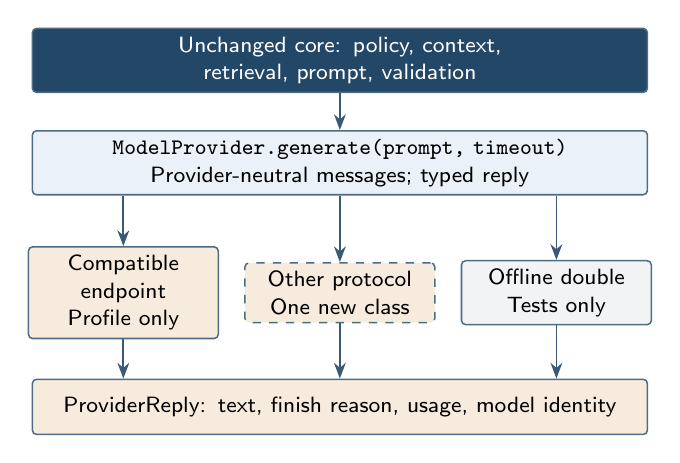
\begin{tikzpicture}
\node[engine,text width=7.6cm] (core) at (0,4.3) {Unchanged core: policy, context, retrieval, prompt, validation};
\node[context,text width=7.6cm] (contract) at (0,3) {\texttt{ModelProvider.generate(prompt, timeout)}\\Provider-neutral messages; typed reply};
\node[external,text width=2.2cm] (http) at (-2.75,1.35) {Compatible endpoint\\Profile only};
\node[external,optional,text width=2.2cm] (native) at (0,1.35) {Other protocol\\One new class};
\node[storage,text width=2.2cm] (stub) at (2.75,1.35) {Offline double\\Tests only};
\node[external,text width=7.6cm] (reply) at (0,-.1) {ProviderReply: text, finish reason, usage, model identity};
\draw[flow] (core) -- (contract);
\draw[flow] (http.north |- contract.south) -- (http);
\draw[flow] (contract) -- (native);
\draw[flow] (stub.north |- contract.south) -- (stub);
\draw[flow] (http) -- (http.south |- reply.north);
\draw[flow] (native) -- (reply);
\draw[flow] (stub) -- (stub.south |- reply.north);
\end{tikzpicture}
\end{document}
